% Options for packages loaded elsewhere
\PassOptionsToPackage{unicode}{hyperref}
\PassOptionsToPackage{hyphens}{url}
%
\documentclass[
  11pt,
  french,
  a5paper,
  openany]{book}
\usepackage{lmodern}
\usepackage{amssymb,amsmath}
\usepackage{ifxetex,ifluatex}
\ifnum 0\ifxetex 1\fi\ifluatex 1\fi=0 % if pdftex
  \usepackage[T1]{fontenc}
  \usepackage[utf8]{inputenc}
  \usepackage{textcomp} % provide euro and other symbols
\else % if luatex or xetex
  \usepackage{unicode-math}
  \defaultfontfeatures{Scale=MatchLowercase}
  \defaultfontfeatures[\rmfamily]{Ligatures=TeX,Scale=1}
\fi
% Use upquote if available, for straight quotes in verbatim environments
\IfFileExists{upquote.sty}{\usepackage{upquote}}{}
\IfFileExists{microtype.sty}{% use microtype if available
  \usepackage[]{microtype}
  \UseMicrotypeSet[protrusion]{basicmath} % disable protrusion for tt fonts
}{}
\makeatletter
\@ifundefined{KOMAClassName}{% if non-KOMA class
  \IfFileExists{parskip.sty}{%
    \usepackage{parskip}
  }{% else
    \setlength{\parindent}{0pt}
    \setlength{\parskip}{6pt plus 2pt minus 1pt}}
}{% if KOMA class
  \KOMAoptions{parskip=half}}
\makeatother
\usepackage{xcolor}
\IfFileExists{xurl.sty}{\usepackage{xurl}}{} % add URL line breaks if available
\IfFileExists{bookmark.sty}{\usepackage{bookmark}}{\usepackage{hyperref}}
\hypersetup{
  pdftitle={Travaux de maturité 2023},
  pdflang={fr},
  hidelinks,
  pdfcreator={LaTeX via pandoc}}
\urlstyle{same} % disable monospaced font for URLs
\usepackage[margin=20mm]{geometry}
\usepackage{longtable,booktabs}
% Correct order of tables after \paragraph or \subparagraph
\usepackage{etoolbox}
\makeatletter
\patchcmd\longtable{\par}{\if@noskipsec\mbox{}\fi\par}{}{}
\makeatother
% Allow footnotes in longtable head/foot
\IfFileExists{footnotehyper.sty}{\usepackage{footnotehyper}}{\usepackage{footnote}}
\makesavenoteenv{longtable}
\usepackage{graphicx,grffile}
\makeatletter
\def\maxwidth{\ifdim\Gin@nat@width>\linewidth\linewidth\else\Gin@nat@width\fi}
\def\maxheight{\ifdim\Gin@nat@height>\textheight\textheight\else\Gin@nat@height\fi}
\makeatother
% Scale images if necessary, so that they will not overflow the page
% margins by default, and it is still possible to overwrite the defaults
% using explicit options in \includegraphics[width, height, ...]{}
\setkeys{Gin}{width=\maxwidth,height=\maxheight,keepaspectratio}
% Set default figure placement to htbp
\makeatletter
\def\fps@figure{htbp}
\makeatother
\setlength{\emergencystretch}{3em} % prevent overfull lines
\providecommand{\tightlist}{%
  \setlength{\itemsep}{0pt}\setlength{\parskip}{0pt}}
\setcounter{secnumdepth}{5}
\usepackage[T1]{fontenc}
\usepackage[]{plex-otf}
\renewcommand*\familydefault{\sfdefault}

\widowpenalty10000
\clubpenalty10000

\renewcommand{\arraystretch}{1.5}

\usepackage{booktabs}
\usepackage{tabto}

\usepackage{fancyhdr}
\setlength{\headheight}{14pt}
\pagestyle{fancy}
\lhead{}
\chead{}
\rhead{\leftmark}
\lfoot{}
\cfoot{\footnotesize\thepage}
\rfoot{}
\renewcommand{\headrulewidth}{0.2pt}
\renewcommand{\footrulewidth}{0.2pt}
\renewcommand{\chaptermark}[1]{\markboth{\footnotesize\space#1}{}}
% \renewcommand{\chaptermark}[1]{\markboth{\footnotesize\thechapter.\space#1}{}}

\fancypagestyle{plain}{
  \setlength{\headheight}{14pt}
  \pagestyle{fancy}
  \lhead{}
  \chead{}
  \rhead{}
  \lfoot{}
  \cfoot{\footnotesize\thepage}
  \rfoot{}
  \renewcommand{\headrulewidth}{0pt}
  \renewcommand{\footrulewidth}{0.2pt}
}

\setcounter{tocdepth}{1}

\usepackage{titlesec}
\titlespacing{\chapter}{0em}{0em}{1em}
\titleformat{\chapter}[display]{\normalfont\bfseries\centering}{}{0pt}{\Large}
\titleformat{\section}[display]{\normalfont\bfseries}{}{0pt}{\large}
\titleformat{\subsection}[display]{\normalfont\bfseries}{}{0pt}{\normalsize}

\newenvironment{signature}{\vspace{2em}\hfill}{}
\ifxetex
  % Load polyglossia as late as possible: uses bidi with RTL langages (e.g. Hebrew, Arabic)
  \usepackage{polyglossia}
  \setmainlanguage[]{french}
\else
  \usepackage[shorthands=off,main=french]{babel}
\fi

\title{Travaux de maturité 2023}
\author{}
\date{\vspace{-2.5em}17.10.2022}

\begin{document}
\maketitle

{
\setcounter{tocdepth}{0}
\tableofcontents
}
\hypertarget{pruxe9ambule}{%
\chapter*{Préambule}\label{pruxe9ambule}}
\addcontentsline{toc}{chapter}{Préambule}

\hypertarget{philosophie-de-lart-la-beautuxe9-et-la-vuxe9rituxe9}{%
\chapter{Philosophie de l'art : La beauté et la vérité}\label{philosophie-de-lart-la-beautuxe9-et-la-vuxe9rituxe9}}

Que la beauté soit une affaire de goût, qu'elle soit subjective, qu'elle soit relative et propre à chacun, c'est ce qui semble aller de soi. Mais que dire du chef-d'œuvre qui prétend à l'universalité~? Que dire du jugement esthétique qui s'offusque lorsqu'on le contrarie~? Une fleur est belle, un paysage est beau, un visage est beau : n'est-ce pas à dire que la beauté se situe dans les choses~? Qu'elle est objective~? Mais alors, comment se dévoile-t-elle~? Est-ce par une modification du regard chez l'observateur, par un travail de l'artiste sur la chose qu'il façonne, ou par l'éclat à peine aperçu d'un objet qui suggère qu'il dissimule un secret~? Pouvons-nous nous contenter de regarder une œuvre d'art ou devons-nous la contempler~? Et l'artiste, dès lors, est-il un créateur ou un voyant~? Il n'est pas rare d'ailleurs que nous ressentions un sentiment d'authenticité face à une œuvre d'art -- comme si là, en face de nous, c'était la vérité qui s'exprimait. Ce sentiment équivaut-il à une émotion~? Une réaction à une réalité qui donne des frissons~? Mais si c'est la vérité qui se manifeste dans une œuvre d'art -- est-ce à dire que la science ne possède pas le monopole du savoir~? Que la science et l'art seraient des disciplines opposées, voire incompatibles~? Rien n'est moins sûr. Mais nous entendons que l'art a pour fonction d'imiter la nature, alors que la science l'explique et la décrit. Ne serait-ce pas que l'art a pour fonction d'embellir la nature~? Mais que dire alors des œuvres sublimes qui accentuent la laideur physique et la dégradation morale de ses sujets~? Que dire des caricatures, par exemple, desquelles se dégagent indiscutablement une modalité du beau et du vrai~? Accentuer les traits, déformer les corps, exagérer les expressions : n'est-ce pas mentir~? Que dire des dissonances musicales qui semblent rompre un ordre harmonique qui est si doux à nos oreilles~? Représenter iconographiquement des êtres célestes et divins, n'est-ce pas profaner des entités qui dépassent la condition de l'homme~? Très rapidement s'est posée la question de savoir comment exprimer une idée artistique.

Nous pourrions en outre nous demander si l'expression artistique est une activité proprement humaine. Ne voyons-nous pas des araignées construire des édifices symétriques, dont la régularité surpassent parfois nos efforts architecturaux~? N'observons-nous pas dans la nature de nombreux actes de séduction animalière qui laissent entendre que les animaux possèdent aussi une sensibilité esthétique~? Peut-être que l'harmonie de la nature nous a conféré des normes artistiques dont il est difficile de nous défaire.

Tel serait un échantillon des questions qui peuvent être soulevées dans ce Travail de Maturité. Avec l'aide de textes appartenant à la tradition philosophique, mais aussi à la littérature, à la poésie, et aux artistes eux-mêmes -- qui ont souvent écrit sur leur pratique --, nous nous interrogerons sur l'attrait qu'exerce sur nous le pouvoir des créations artistiques. Qu'il s'agisse du plaisir indescriptible qu'éveille la jouissance artistique, du moment de suspens que provoque en nous l'expérience esthétique elle-même, du basculement par lequel nous nous perdons dans un tableau, dans une sculpture, dans un morceau de musique, ou dans un film, du sérieux ou du jeu avec lesquels nous nous approchons d'une œuvre d'art, du milieu dans lequel l'œuvre d'art doit ou peut être appréhendée (théâtre, musée, chez soi, nature), de la modification que lui fait subir les impératifs de consommation, nous nous attacherons à montrer que la création artistique possède une place fondamentale dans notre rapport au monde.

\clearpage

Ce Travail de Maturité est ouvert à tous et n'exige aucun prérequis. Il demande simplement un intérêt pour la question artistique, une envie de penser, et une dose de curiosité.

\begin{signature}
Jeremy Filthuth et Esma Puric

\end{signature}

\hypertarget{le-ruxe9cit-de-voyage}{%
\chapter{Le récit de voyage}\label{le-ruxe9cit-de-voyage}}

\begin{figure}

{\centering 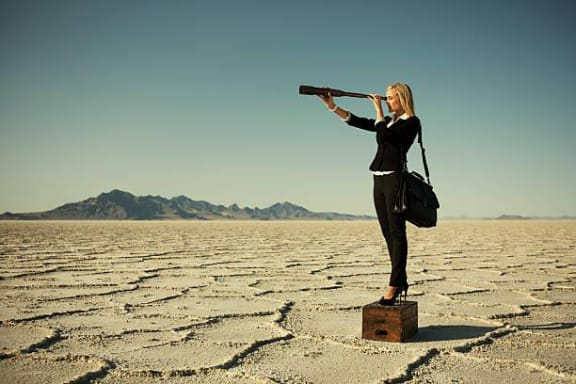
\includegraphics[height=12em]{images/le-recit-de-voyage} 

}

\end{figure}

De tous temps, nous, humains, avons ressenti l'appel du large et sommes partis à l'aventure vers des contrées inconnues pour en rapporter des histoires fantastiques. Le voyage permet de sortir de nos habitudes, de retrouver l'essentiel et parfois de nous donner l'illusion de la liberté.

Dans ce TM il s'agira de choisir votre propre destination pour ensuite en faire un récit de voyage. Nous aborderons le récit de voyage à travers des auteurs comme Sylvain Tesson, Ella Maillart ou d'autres écrivains. Puis ça sera à vous, par groupe de deux, d'organiser puis d'entamer votre voyage qui constituera la base de votre récit. Nul besoin d'aller à l'autre bout de la planète : il s'agit de sortir de son quotidien et de sa zone de confort et de partir à la découverte de lieux nouveaux qui nourrissent notre imaginaire. Vous en ferez ensuite votre propre récit de voyage, un texte écrit et agrémenté par exemple de photos, de vidéos ou de dessins pour à votre tour faire voyager vos lecteurs.

N.B. Ce TM peut se faire en français ou en anglais et doit être rédigé à deux.

\hypertarget{travel-literature}{%
\section*{Travel literature}\label{travel-literature}}
\addcontentsline{toc}{section}{Travel literature}

For ages, we have felt the call from the sea and have adventured towards unknown places coming back to narrate our incredible experiences. Traveling allows us to escape from our habits, find what's essential and sometimes gives us the illusion of being free.

In this TM you will discover what travel literature is, through texts by Sylvain Tesson, Ella Maillart or other writers. Then it will be your turn, in groups of two, to organise and start off your own travel adventure which will be the starting point of your text. No need to go far away: it's about leaving our daily routine and comfort zone to discover new places that fuel our imagination. You will then produce a written text on your travel adding for example photos, videos and drawings to make your readers travel as well.

N.B. This TM can be written in French or English and needs to be done in groups of two.

\begin{signature}
Jasmine Menamkat

\end{signature}

\hypertarget{le-jeu-viduxe9o-fiction-ou-ruxe9alituxe9}{%
\chapter{Le jeu vidéo : fiction ou réalité~?}\label{le-jeu-viduxe9o-fiction-ou-ruxe9alituxe9}}

\begin{figure}

{\centering 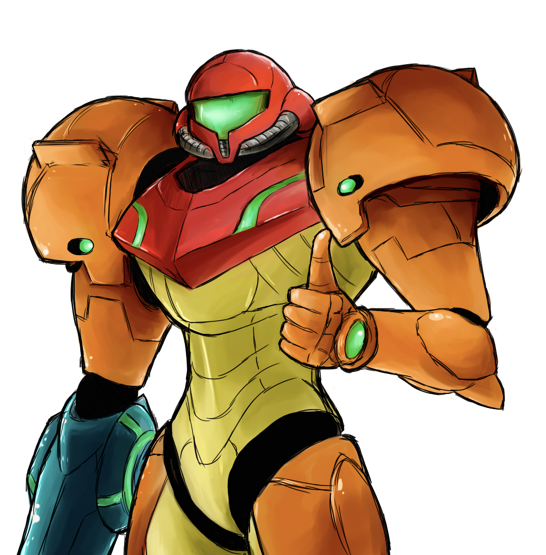
\includegraphics[height=12em]{images/le-jeu-video-fiction-ou-realite} 

}

\end{figure}

Depuis une dizaine d'années, la pratique du jeu vidéo s'est répandue à une large partie de la population. Bien que de nombreuses personnes aient accusé ce divertissement d'être à l'origine de violences ou de provoquer l'isolement des gameurs-euses, nous parlons actuellement du 10\textsuperscript{e} art pour nommer les jeux vidéo.

La stratégie de cette industrie ne repose pas uniquement sur le degré de divertissement qu'ils procurent, mais également sur leur impact visuel comme intellectuel. Ainsi a-t-on réalisé d'impressionnants progrès dans le développement réaliste des graphiques et dans la complexité de leur scénario.

Tout en laissant place à des produits originaux et conceptuels, les développeurs-ses tendent donc à mêler le réel à la fiction en ouvrant le champ à de nouvelles réflexions : comment représenter la société, le genre, la femme~? Comment simuler l'histoire, la gestion, les métiers~? Comment vous permettre à vous, gameurs-euses, de vous plonger dans un divertissement si immersif qu'il vous ouvre les portes d'une nouvelle dimension~?

La finalité de ce travail de maturité est d'étudier la limite entre la réalité et la fiction dans le jeu vidéo. Ce sujet, vaste, vous laisse donc la liberté de proposer diverses problématiques faisant appel à votre pratique, hautement recommandée, des jeux vidéo.

\begin{signature}
Alan Morier et Loïc Moser

\end{signature}

\end{document}
